\subsection{Warstwa antyrefleksyjna}
\begin{figure}[tb]
	\centering
        \begin{subfigure}{0.42\textwidth}
		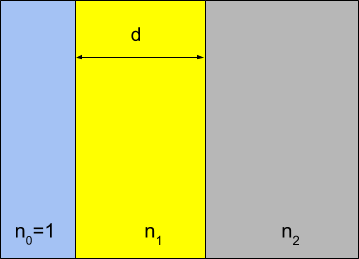
\includegraphics[width=\textwidth]{images/pml/antiref.png}
                \caption{}
		\label{fig:antyref}
        \end{subfigure}
        \begin{subfigure}{0.47\textwidth}
                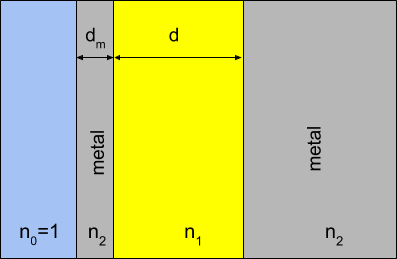
\includegraphics[width=\textwidth]{images/pml/sailsbury.png}
                \caption{}
		\label{fig:sailsburyschem}
        \end{subfigure}
        \caption{(a) Schemat prostej warstwy antyodbiciowej  (b) Płytka absorbująca Salisburego}
\end{figure}



\begin{figure}[tb]
	\centering
	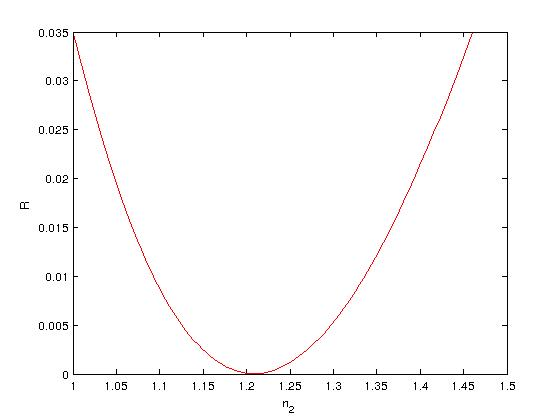
\includegraphics[width=0.9\textwidth]{images/antyref.jpg}
	\caption{Zależność współczynnika odbicia od współczynnika załamania warstwy antyrefleksyjnej dla warstwy o grubości $d=\frac{\lambda_0}{4 n_1}$ umieszczonej pomiędzy powietrzem, a~materiałem o~współczynniku załamania $n_3=1.5$}
	\label{fig:antyref-result}
\end{figure}


Działanie prostych absorberów elektromagnetycznych jest analogiczne do warstwy antyodbiciowej. Rozważmy   warstwę antyodbiciową przedstawioną na rysunku \ref{fig:antyref}. Na granicy powietrza i dielektryka o współczynniku załamania $n_2$ wprowadziliśmy warstwę innego dielektryka o~współczynniku załamania $n_1$, takim że $1<n_1<n_2$. Dokładne wartości współczynnika odbicia od obu granic ośrodków możemy obliczyć za pomocą równań Fresnela. Dla prostoty skupmy się na szczególnym przypadku padania normalnego. Natężeniowy współczynnik odbicia od granicy powietrza i ośrodka o współczynniku załamania $n_2$ wynosi:
\begin{equation}
R=\bigg|\frac{1-n_2}{1+n_2}\bigg|^2.
\end{equation}
Jeżeli jednak pomiędzy powietrze i dielektryk wprowadzimy dodatkową warstwę, wtedy natężeniowy współczynnik odbicia od takiego układu wyraża się wzorem
\begin{equation}
R=\Bigg| \frac{r+r' exp(2 i\phi)}{1+r r' exp(2 i\phi)} \Bigg|^2,
\end{equation}
w którym $r$ i $r'$ oznaczają odpowiednie amplitudowe współczynniki odbicia od granicy ośrodków wynikające z wzorów Fresnela:
\begin{equation}
r=\frac{1-n_1}{1+n_1},
\end{equation}
\begin{equation}
r'=\frac{n_1-n_2}{n_1+n_2},
\end{equation}
a $\phi$ oznacza zmianę fazy fali E-M w trakcie propagacji przez dodatkową warstwę. Zmiana fazy dla kierunku padania światła prostopadłego do powierzchni warstw wyraża się przez $\phi=k_0 d n_1$, gdzie $k_0$ jest liczbą falową, a $d$ grubością warstwy antyodbiciowej, natomiast ogólniej, dla padania ukośnego $\phi=k_y d$, gdzie $k_y$ jest składową wektora falowego wewnątrz warstwy antyodbiciowej, normalną do granicy warstw. 

 W ten sposób uzyskaliśmy układ, dla którego współczynnik odbicia jest mniejszy niż współczynnik odbicia od półprzestrzeni wypełnionej materiałem, o współczynniku załamania $n_2$. Zależność współczynnika odbicia od układu z warstwą antyrefleksyjną w zależności od współczynnika załamania $n_1$ dla $n_2=1.46$ przedstawia wykres na rysunku \ref{fig:antyref-result}. Współczynnik odbicia przyjmuje zerową wartość współczynnika załamania $n1$ warstwy antyrefleksyjnej równej średniej geometrycznej ze współczynników załamania ośrodków zewnętrznych $n_1=\sqrt{n0\textrm{ }n2}$, czyli gdy $r=r'$ oraz dla odpowiednio dobranej grubości $d$.

Podstawowym mechanizmem, wykorzystywanym w konstrukcji warstw antyodbiciowych jest interferencja. Dobranie grubości $d=(1+2m)\frac{\lambda_0}{4 n_1}$, gdzie $\lambda_0$ to długość fali w próżni, a $m$ dowolną liczbą całkowitą prowadzi do destruktywnej interferencji między falami odbitymi od pierwszej i drugiej granicy ośrodków. Matematycznie oznacza to spełnienie warunków $exp(2 i \phi)=-1$, a w konsekwencji $R=0$ dla długości fali $\lambda_0$. Powstałe w ten sposób minimum współczynnika odbicia $R=0$, występuje dla wąskiego zakresu długości fali. Możliwe jest uzyskanie niskiego współczynnika odbicia dla szerokiego zakresu długości fali poprzez dodanie kolejnych warstw, o innej grubości optycznej~\cite{poitras2004toward}. Współczynniki załamania w tak zbudowanej strukturze mogą w szczególności zmieniać się zgodnie z postępem geometrycznym $n_i^2=n_{i-1} \cdot n_{i+1}$, a grubość każdej z warstw musi spełniać warunek $d_i=\frac{\lambda_0}{4 n_i}$~\cite{pochi1988optical}. Projektując takie struktury możliwe jest uzyskiwanie powierzchni o wybiórczym, ze względu na częstotliwość, współczynniku odbicia~\cite{monacelli2005infrared}. 

\subsection{Ekran Salisbury'ego}
Również na zasadzie interferencyjnego wygaszenia odbicia~\cite{us1952absorbent}, działa prosty absorber przedstawiony na rysunku \ref{fig:sailsburyschem}. Przed powierzchnią metalu w odległości $d$ znajduje się cienka warstwa metalu. Grubość warstwy $d_m$ musi być porównywalna z grubością naskórkową, aby umożliwić transmisję fal E-M przez tę warstwę. W ten sposób pomiędzy zwierciadłem, a cienką warstwą o grubości $d_m$ powstaje wnęka. Zazwyczaj tłumienie wprowadza się za pomocą urojonej części współczynnika załamania $n_1$, możliwe jest jednak oparcie tłumienia jedynie na stratach związanych z grubą warstwą metalową tworzącą zwierciadło. 

\begin{figure}[tb]
	\centering
	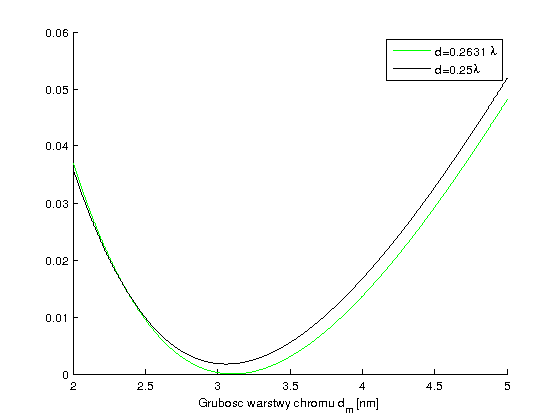
\includegraphics[width=\textwidth]{images/pml/sailsbury-res.png}
	\caption{Zależność natężeniowego współczynnika odbicia od grubości warstwy metalowej $d_m$, dla grubości warstwy o współczynniku załamania $n_2=3.34 + 4.27i$ równiej odpowiednio $d=0.2631\lambda_0$ i $d=0.25\lambda_0$}
	\label{fig:sailsburyres}
\end{figure}

Jako przykład,  wykres na rysunku \ref{fig:sailsburyres}  przedstawia zależność współczynnika odbicia od układu przedstawionego na rysunku \ref{fig:sailsburyschem} dla padającego promieniowania o długości fali $\lambda_0$=633~nm w zależności od $d_m$. Jako współczynnik załamania w cienkiej warstwie metalowej przyjęto $n_2=3.34+4.27i$ co odpowiada własnościom chromu dla rozważanej długości fali~\cite{ordal1983optical}. Dobranie odpowiedniej odległości $d$ i grubości warstwy chromu $d_m$ pozwala na wytworzenie warunków destruktywnej interferencji umożliwiając uzyskanie zerowego współczynnika odbicia. W wyniku odbicia na granicy ośrodków o współczynnikach załamania $n_1$ i $n_2$ wprowadzane jest również przesunięcie fazy. Konieczność skompensowania tego przesunięcia, jak i skończone rozmiary warstwy półprzepuszczalnej $d_m$ powodują, że optymalna grubość materiału o współczynniku załamania $n_1$ nieco odbiega od $\frac{\lambda_0}{4 n_1}$, co ilustrują wyniki na rysunku \ref{fig:sailsburyres}. 

\subsection{Inne propozycje realizacji absorberów}

Innym podejściem jakie można spotkać w literaturze jest wytworzenie warstw nieodbijających za pomocą cienkiej warstwy ferro- i ferimagnetyków tworzących  statyczną magnetyzację o charakterze periodycznym   \cite{ramprecht2008scattering}. Autorzy prezentują wyniki symulacji dowodzące możliwości uzyskania współczynnika odbicia poniżej -20dB w~zakresie od 1 do 4 GHz, niezależnie od kąta padania. W~ostatnich latach proponowane były również absorbery oparte na rezonatorach SRR~(ang.~split-ring resonator), w których warstwa nieodbijająca jest realizowana poprzez uzyskanie dopasowania impedancyjnego z powietrzem jednocześnie wykorzystują stratność w metamateriale. Omówienie prac wykorzystujących tę technikę  można znaleźć w~artykule~\cite{watts2012metamaterial}.

Imponujące wyniki eksperymentalne pozwalające uzyskać wysoki współczynnik absorpcji w szerokim zakresie spektralnym zostały uzyskane za pomocą lasów nanorurek węglowych \cite{mizuno2009black}. Zaprezentowane przez autorów wyniki eksperymentalne wskazują na współczynnik odbicia mniejszy niż 2\% w zakresie od 200~nm do 20µm.

Możliwa jest również konstrukcja absorberów wykorzystujących wielowarstwy metaliczno-dielektryczne. Tego typu absorbery osiągają współczynnik absorpcji większy niż 80\%, dla całego zakresu długości fali ciała doskonale czarnego o temperaturze 300K~\cite{guo2014impact,corrigan2012broadband}. Autorzy dyskutują w pracy dalsze możliwości zmniejszenia współczynnika odbicia poprzez wprowadzenie dodatkowej porowatej warstwy antyodbiciowej. 

W kolejnych podrozdziałach przedstawiona zostanie inna możliwa do zastosowania koncepcja umożliwiająca uzyskanie warstwy charakteryzującej się niskim współczynnikiem odbicia w szerokim zakresie długości fali i kątów padania. 
